\chapter{Understanding Robotic Visual Semantic Navigation}\label{ch:understanding-robotic-visual-semantic-navigation}

%Describe motivation of the problem (navigation is important for robots)
\lettrine{\textcolor{accent_color}{O}}{ne} of the most important tasks that humans perform in their daily lives is semantic and goal-oriented navigation.
This ability to navigate like a human towards a target in the environment is considered one of the ``holy grail'' goals of intelligent robots.
There are countless applications that could be supported by a robotic platform with this capacity.
From assistive robots that can accompany a person to perform a specific task, to platforms that navigate autonomously in complex work environments, such as logistics centers.

%Describe the problem of visual semantic navigation (briefly)
This chapter addresses the problem of \acrlong{vsn}.
The goal is to make a robot capable of navigating through an environment to reach a particular object (the target) in the surroundings, such as a chair, mainly using vision-based sensors.
Technically, a \acrshort{vsn} approach is a learning-based navigation model, where no geometry-based traditional techniques are applied.
Nor the map of the environment is known a priori, neither the map is built on the fly.
The majority of methods integrate \acrshort{rl} techniques with current developments in deep learning models for visual perception.

\begin{figure}
    \centering
    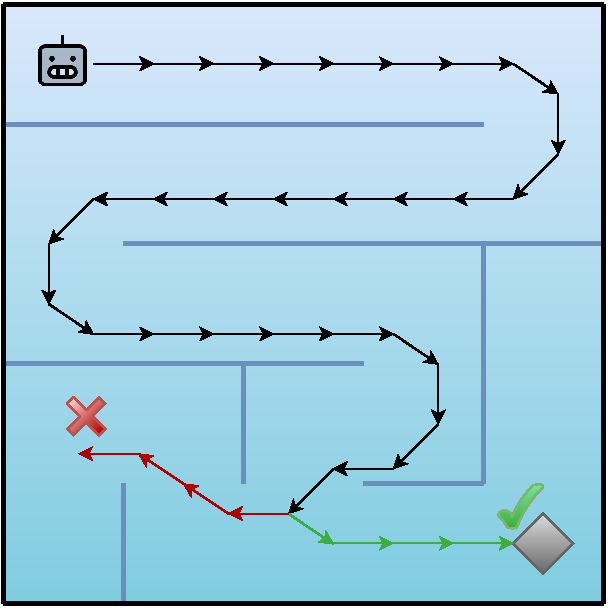
\includegraphics[width=0.6\linewidth]{figures/understanding_vsn/graphical_abstract}
    \caption{Can an agent pinpoint a target in a maze using a \acrshort{vsn} model based on state-of-the-art RL and deep learning models? This chapter explores and analyzes the solutions for the main challenges in \acrshort{vsn}, \ie unknown environments, visibility of targets and path planning.}
    \label{fig:graphical_abstract}
\end{figure}

%Describe the problem we address (use the graphical abstract)
The main questions this chapter addresses are: Is it possible to offer accurate experimental evaluation settings so that different \acrshort{rl}-based \acrshort{vsn} models may be clearly compared to one another?; What are the main challenges associated with these \acrshort{rl}-based \acrshort{vsn} models?
With respect to the former, after reviewing the literature, it is difficult to make direct comparisons between the many solutions provided.
The key challenges are that the navigation settings in which the experimental metrics are given are not available, and that each technique employs a separate set of \acrshort{rl} libraries.
With respect to the second question, three are the main challenges that every \acrshort{vsn} model needs to tackle.
See Figure~\ref{fig:graphical_abstract}.

Is it possible for an agent to localize a target in a maze with a \acrshort{vsn} model based on state-of-the-art deep learning and \acrshort{rl} models?
To begin with, it must be taken into consideration that the environment is, or might be, unknown to the agent.
The experiments expose the agent to different mazes.
In this situation, the robot would need to explore the environment to learn more about it.
Second, how does the agent deal with the visibility of the targets?
For a \acrshort{vsn} model, the object it has to navigate to may not be visible at the beginning or during navigation.
How does the agent learn a search strategy to find the object in the maze?
And third, even if the target is visible, the robot must devise a feasible route to reach it.

The main contributions of this chapter are as follows:
\begin{enumerate}
    \item A \acrshort{vsn} model which leverages state-of-the-art \acrfull{clip} encoders~\cite{radford2021}.
    Technically, it is a model that combines a \acrshort{clip} encoder with a set of two \acrshort{rnn}s for producing the discrete navigation actions that the agent needs to take (Section~\ref{sec:navigation}).
    \item The agent is trained following a \acrshort{rl} paradigm for \acrshort{vsn}.
    This work evaluates the impact of each of the \acrshort{vsn} challenges mentioned above, using different techniques that have been proposed in the literature: reward shaping~\cite{sutton2018, wijmans2020} to deal with the sparsity of the reward signal naturally associated with the navigation problem; and $\epsilon\text{-}greedy$~\cite{mnih2013} as a mechanism to balance exploitation and exploration.
    \item A thorough experimental evaluation setup has been designed (Section~\ref{sec:experiments}) with the aim to offer a clear experimental environment in which to compare different \acrshort{vsn} approaches.
    It has been implemented using pyRIL~\cite{pyRIL}, an open source python library for \acrshort{rl}, and two navigation environments: a maze navigation setup of Miniwolrd-Maze from \textit{gym-miniworld}~\cite{gym_miniworld}; and a navigation through a 3D photorealistic scan indoor space provided by \acrshort{hm3d} dataset~\cite{ramakrishnan2021} in Habitat~\cite{szot2021} simulator.
    The codes to reproduce the experiments are released, as well as the whole experimental setup, so that others can compare their work with these results.
\end{enumerate}


\section{RL For Navigation}\label{sec:navigation}

\subsection{Problem Formulation}\label{subsec:problem-formulation}

This chapter addresses the \acrshort{vsn} problem by using \acrshort{rl}.
Thus, navigation can be described as a \acrfull{pomdp}, in which the agent, \ie a robot, navigates through an environment and tries to reach a determined object.
This problem is known in the literature as the \acrfull{objnav} task~\cite{batra2020}.

Formally, given an initial observation distribution $p_0$, for the step $t$ the agent receives an observation $o_t \sim p_0(o)$ based on state $s_t$, which in this case is just an RGB image of what the robot observes.
The agent takes action $a_t$, obtains reward $r_t$ from the environment and receives a new observation $o_{t+1} = \mathcal{T} (o_{t+1}|o_t, a_t)$, where $\mathcal{T}$ is the transition function.
An episode is a sequence of $\left(o_t, a_t, r_t\right)$ tuples that form a trajectory.
The episode ends when the agent reaches the goal or the maximum number of steps ($H$).
An episode is considered a success if the agent reaches the goal within the step horizon $H$.

The goal is to find an optimal policy $\pi^*$ that maximizes the cumulative reward over an episode.
This policy maps observations to a probability distribution over actions that is specified as follows,
\begin{equation}
    \label{eq:op_policy}
    \pi^*=\argmax\limits_\pi\mathbb{E}_{\mathcal{T}\sim\pi}[R_H],
\end{equation}
where $R_H=\sum_{t=1}^H \gamma^{t-1}r_t$ is the return, \ie the cumulative reward over an episode, and $\gamma$ is a discount factor.
In navigation tasks, neural networks with parameters $\theta$ are often used to parameterize the policy $\pi_\theta$.

\subsection{Visual Semantic Navigation}\label{subsec:visual-semantic-navigation}

Learning to navigate in a given environment is a challenging task.
First, the reward signal coming from the environment is usually sparse~\cite{sutton2018, pathak2017}.
These sparse rewards lead to a quite difficult training process.
%Second, the agent has to balance an exploration of the environment to obtain experience and the exploitation of the previous experience in order to obtain successful episodes~\cite{sutton2018, mnih2013}.
Second, it is necessary to find a balance between the exploration and exploitation of the environment to achieve successful experiences that drive the agent's learning process~\cite{sutton2018, mnih2013}.
Finally, the agent architecture has a direct impact on how it learns.
State-of-the-art approaches use a feature extractor followed by recurrent units to process temporal information coming from the images.
%For navigation tasks, a common agent architecture consists of a CNN feature extractor and an RNN that outputs the action distribution.

\textbf{Sparse rewards and long horizon.}
%In visual navigation, sparse rewards are a common issue due to the nature of the task, \ie reaching a specific target in an environment.
Sparse rewards are a common issue due to the nature of the navigation tasks, \ie reaching a specific target in an environment.
The most straightforward way to define a reward in navigation problems is to let the environment provide a fixed amount when the agent reaches the goal.
This means the agent has to face an environment in which:
1) in the best case, most of the reward signal is zero except for the step in which the agent reaches the goal and obtains a certain amount of reward;
and 2) if the agent does not reach the target, it does not receive any reward.
This situation worsens with large temporal horizons, because the more steps, the higher the sparsity of the reward is.

To mitigate the sparse reward problem, this approach uses a technique called reward shaping.
It consists in modifying the original reward signal via incorporating domain knowledge.
For navigation, the approach leverages on the \textit{distance reward}~\cite{wijmans2020}, defined as:
\begin{equation}
    \label{eq:rew_shaping}
    r_t = -d(s_t, target) + d(s_{t+1}, target) - r_s + r_T,
\end{equation}
where $d(s_t, target)$ computes the geodesic distance between agent's position at state $s_t$ and the $target$ position.
$r_T$ is the \textit{terminal reward}, a fixed amount given only when the agent reaches the target and $r_s=0.01$ is the \textit{slack reward}, also a fixed amount that penalizes each step.
The goal of the \textit{distance reward} function is to give a constant reward signal to the agent that increases as the agent approaches the target.
In section~\ref{subsec:miniworld-maze-results} the \textit{distance reward} is compared against what is usually referred to as the \textit{navigation reward}, which consists only of the slack reward and the terminal reward $r_t = -r_s + r_T$.

\textbf{Exploration vs. Exploitation.}
As previously mentioned, the exploration process has to be managed to encourage the agent to choose actions that it would not otherwise select.
To address this issue, the study leverages the technique known as $\epsilon\text{-}greedy$~\cite{mnih2013}.
This solution \emph{controls} the action that is being selected by the agent, usually during the learning process.
Given an $\epsilon \in [0, 1]$, an action $a_t$ is selected as
\begin{equation}
    \label{eq:eps-greedy}
    a_t = \begin{cases}
              \argmax\pi_\theta & \mbox{with probability 1-$\epsilon$,}     \\
              rand(a) \in \mathcal{A} & \mbox{with probability $\epsilon$,} \\
    \end{cases}
\end{equation}
where $\mathcal{A}$ defines the action space.
Typically, $\epsilon$ starts at $1$ and it decays with the iterations.
In the beginning of the learning process, \ie when $\epsilon$ is high, random actions are sampled more often, encouraging the agent to explore the environment.
As the training process advances, lower $\epsilon$ values permit the agent to exploit the model knowledge to select the best action.
This introduces a balance between exploration and exploitation.

\textbf{Agent architecture.} The agent is encoded as a parameterized model consisting of a \acrshort{clip}~\cite{khandelwal2022} visual encoder connected to two actor-critic \acrfull{lstm} that output a discrete distribution over the action space and the value, respectively.
A diagram of the implemented agent can be found in figure~\ref{fig:network_clip_diagram}.
To train the models, \acrfull{ppo}~\cite{schulman2017}, an on-policy \acrshort{rl} algorithm, is used.

\begin{figure}
    \centering
    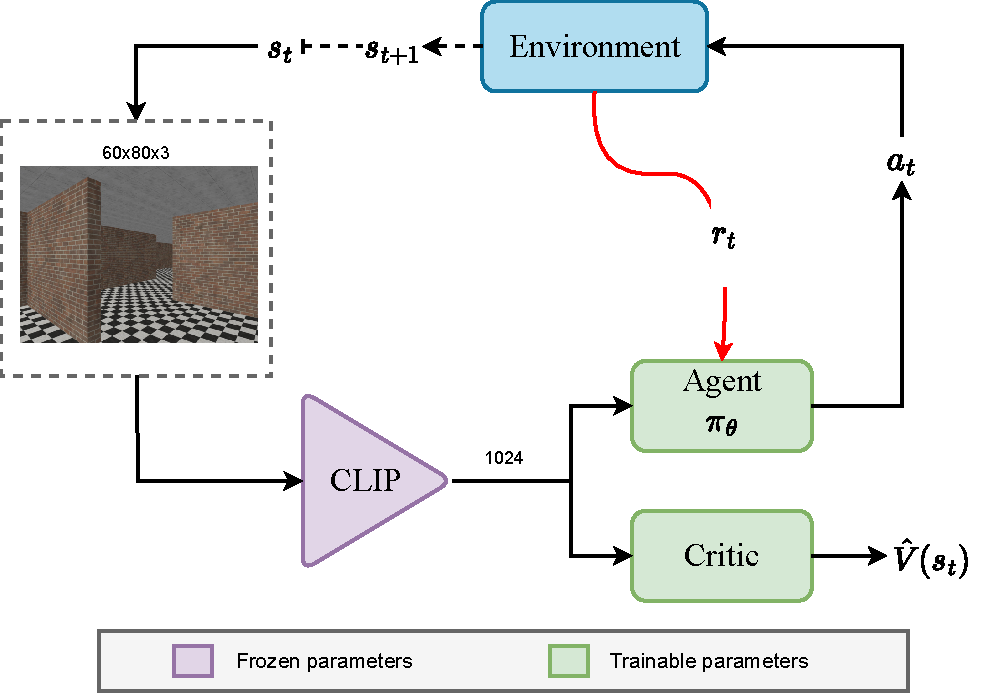
\includegraphics[width=\linewidth]{figures/understanding_vsn/network_clip_diagram}
    \caption{\textbf{Model diagram}. This figure contains a high-level representation of the model used: a visual encoder followed by an actor-critic module encoded by \acrshort{lstm}s. The visual encoder is frozen, and only the actor-critic module is trained.}
    \label{fig:network_clip_diagram}
\end{figure}


\section{Experiments}
\label{sec:experiments-vsn-understanding}

%List of questions that we want to answer.
The experiments in this chapter aim to answer the following questions:
\begin{enumerate}
    \item How does a state-of-the-art navigation model (\acrshort{clip} + \acrshort{lstm} + \acrshort{ppo}) behave in a not-so-complex maze-based environment?
    See section~\ref{subsec:miniworld-maze-results}.
    \item What is the real impact of reward shaping and $\epsilon\text{-}greedy$ techniques on such a model?
    See section~\ref{subsec:miniworld-maze-results}.
    \item When faced with a more realistic robotic navigation scenario, such as the one proposed with HM3D~\cite{ramakrishnan2021} dataset scenes in Habitat~\cite{szot2021}, what is the performance of the model under analysis?
    \item Qualitatively, how does the model navigate through the proposed environments?
    \item Is it feasible to provide clear experimental comparison environments to establish benchmarks between different \acrshort{rl}-based visual semantic navigation models?
\end{enumerate}

\subsection{Experimental setup}\label{subsec:experimental-setup}

\paragraph*{Navigation benchmarks}

The main experimentation was conducted in the Miniwolrd-Maze environment from \textit{gym-miniworld}~\cite{gym_miniworld}.
This is a minimalistic 3D interior environment simulator for \acrshort{rl} and robotics, where 3D mazes can be procedurally generated.
In this benchmark, the agent receives an egocentric 3D view of the environment and has to navigate to a red cube representing the target.
A schematic top-view representation can be found in figure~\ref{fig:graphical_abstract}.
Two configurations are proposed, Maze-S3 and Maze-S5, that correspond to $3\times3$ and $5\times5$ tile maze environments, respectively.
The agent and the target are initialized in opposite corners of the Maze, and in every episode, a new wall distribution is randomly generated.
The action space $\mathcal{A}$ consists of the following actions: $move\_forward$, $turn\_left$, $turn\_right$.
To establish future comparisons with new navigation models in this benchmark, 100 procedurally generated mazes are provided and used as a separate test set.


The second environment is Habitat~\cite{szot2021}, which allows for the training of embodied \acrshort{ai} agents, such as virtual robots, in a highly photorealistic and efficient 3D simulator.
This scenario is particularly relevant because it allows for the evaluation of how a robot would behave in a more realistic navigation scenario than the one posed with the mazes.
One 3D scene from \acrshort{hm3d}~\cite{ramakrishnan2021} dataset is used (see figure~\ref{fig:dollhouse}).
%This dataset consists of 3D reconstructions from real-world locations and posses state-of-the-art visual fidelity.
An \textit{oracle stop} configuration is followed in Habitat, in which the environment is in charge of telling the agent when to stop, so the action space $\mathcal{A}$ consists of the following actions: $move\_forward$, $turn\_left$, $turn\_right$, $look\_up$ and $look\_down$.

As for the evaluation metrics, the Maze models are evaluated using \acrfull{sr} and \acrfull{spe} metrics.
Additionally, for Habitat models, \acrfull{spl} and \acrfull{dtg} metrics are also employed.
All these are the standard metrics for the \acrshort{objnav} problem in Habitat Challenge~\cite{batra2020}.

\paragraph*{Implementation details}
%Provide the details of the benchmark we propose: description of PyRIL, models for navigation, implementation details that can help others to replicate/understand the results.
This work leverages on the state-of-the-art \acrshort{rl} approach for embodied navigation in~\cite{khandelwal2022} with some minor simplifications.
As it is shown in figure~\ref{fig:network_clip_diagram}, the first part of the model consists of a pre-trained \acrshort{clip} plus RestNet50 module as feature extractor, which receives an RGB image and produces a latent vector of size 1024.
The embeddings for the last 10 time steps are then computed and passed through a \acrshort{lstm} layer with 128 neurons.
Finally, two hidden linear layers of 128 neurons with a tanh unit for activation are concatenated.
The agent has two separate networks, one for the actor and one for the critic.
Both networks share the feature extractor.
The output layer of the actor consists in a linear layer of the same dimension as the number of actions with a softmax function.
The output layer of the critic consists of a linear layer with one neuron and linear activation.

The \acrshort{ppo}~\cite{schulman2017} agent provided by pyRIL reinforcement learning library~\cite{pyRIL} is used.
This is a lightweight python library which contains a collection of state-of-the-art deep reinforcement and imitation learning methods, environment wrappers, modularity and different prototyping options.

As the codes are publicly released, a set of tools is provided to improve the reproducibility of \acrshort{rl} experiments, with clear and standardized evaluation protocols.
% \begin{itemize}
%     \item Providing a standard ecosystem for those starting out in embodied navigation with reinforcement learning.
%     \item Provide new set of tools that helps to reproducibility of experiments.
%     \item Provide a standardized evaluation set for Maze.
%     \item Provide standardized metrics as success rate and SPL to evaluate agents performance on Habitat environments.
% \end{itemize}

\subsection{Miniworld-Maze results}\label{subsec:miniworld-maze-results}

First, this section examines how the state-of-the-art \acrshort{clip} + \acrshort{lstm} model behaves in the Miniworld-Maze environment.
Learning curves for Maze-S3 and Maze-S5 are shown in figure~\ref{fig:reward-maze-results}.
These learning curves correspond to the best model, \ie, a model trained with an $\epsilon\text{-}greedy$ strategy and \textit{distance reward} (defined in section~\ref{subsec:visual-semantic-navigation}).
It can be observed how on Maze-S3 the agent rapidly figures out how to resolve the maze in most cases, even getting a good reward from the beginning.
On the other hand, the Maze-S5 learning curve shows that it is a more challenging scenario.
The maze is bigger, so the distance that the agent has to travel in order to reach the target is larger, as well as the number of paths to explore.
This translates into a slower learning curve that takes significantly more time to achieve its peak reward.


The performance of the models in the proposed test set is reported in table~\ref{tab:results-maze}.
A comparison is made between two output strategies of the model to generate the actions:
1) using $\epsilon\text{-}greedy$ with $\epsilon=0.2$ during the evaluation;
and 2) sampling a \textit{stochastic} action from the final layer weights of the agent as a probability distribution.
A random agent is also included as a control case.
Both output options obtain the best results using $\epsilon\text{-}greedy$ exploration in the two mazes.
This fact can be explained by considering how the $\epsilon\text{-}greedy$ exploration is treated during training.
At the beginning of the training process $\epsilon$ starts at a value of $1$ and is annealed until a final value of $0.2$, the same value used for evaluation.
It can also be seen that the model achieves three times more success in Maze-S3 than in Maze-S5.
This indicates that larger mazes are more challenging and need specific learning mechanisms.

To study the impact of reward shaping and $\epsilon\text{-}greedy$ techniques, an ablation study is performed as shown in table~\ref{tab:ablation-study} and figure~\ref{fig:ablation-maze-success}.
The best results are obtained when \textit{distance reward} and $\epsilon\text{-}greedy$ techniques are combined, which demonstrates that both components are important in order to navigate in large environments.
Note that this analysis is done in the S5 mazes.
When only the \textit{distance reward} technique is used, its performance is not enough to make the agent navigate, achieving only a 2\% of success rate.
On the other hand, just using the $\epsilon\text{-}greedy$ strategy, the model achieves a better performance by itself, indicating that in a Maze environment it is key to explore to find the correct path to the target.
Figure~\ref{fig:maze_qualitative} shows the importance of the $\epsilon\text{-}greedy$ technique.
When the agent reaches a corner near the target (red square), it can get stuck and run out of steps (figure~\ref{fig:maze_qualitative_fail}), but using the $\epsilon\text{-}greedy$ technique lets the agent continue exploring.

\begin{figure}
    \centering
    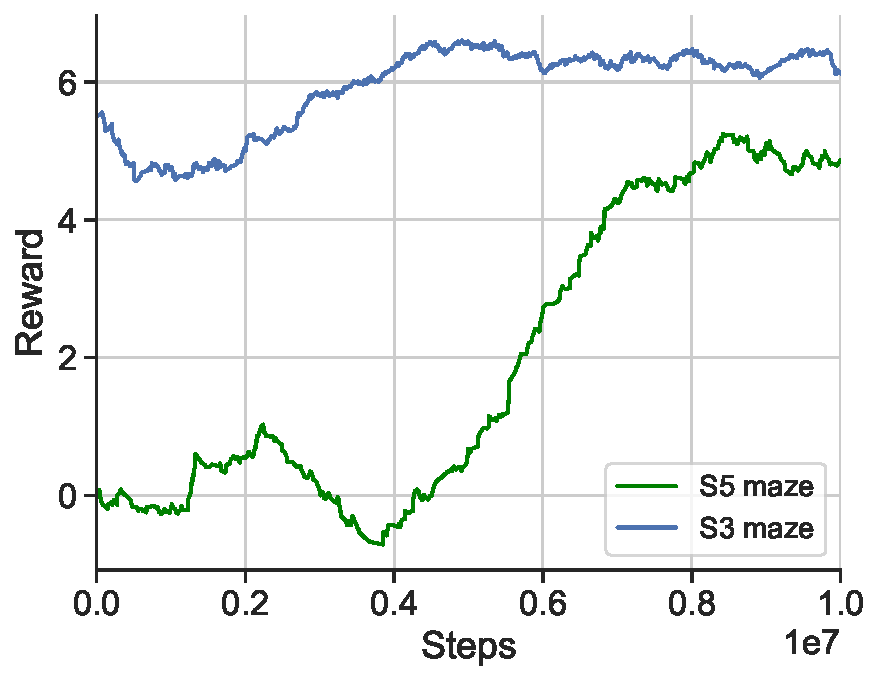
\includegraphics[width=0.8\linewidth]{figures/understanding_vsn/S3_S5_reward}
    \caption{\textbf{Learning curves for Maze-S3 and Maze-S5.} These curves show that the bigger the maze, the higher the complexity. On Maze-S3 the agent already starts at the saturation value around 6.5, but for Maze-S5 the agent needs more steps until it reaches its peak reward around a value of 5.}
    \label{fig:reward-maze-results}
\end{figure}

\begin{figure}
    \centering
    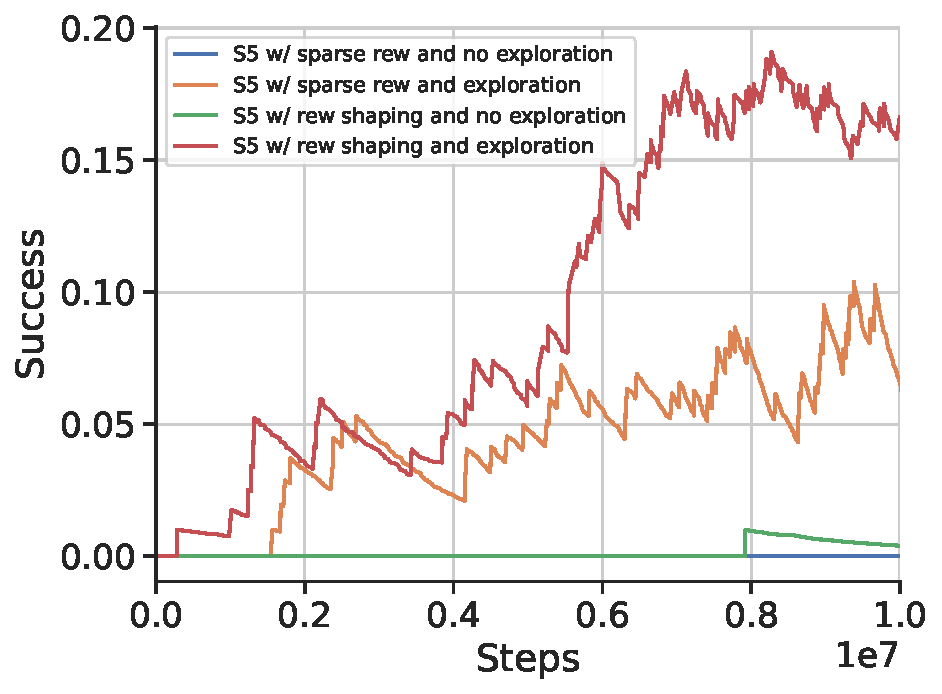
\includegraphics[width=0.8\linewidth]{figures/understanding_vsn/S5_ablation_success}
    \caption{\textbf{Ablation study on Maze-S5 during learning process.} Curves show that the best success rate is obtained using reward shaping and exploration techniques.}
    \label{fig:ablation-maze-success}
\end{figure}

\begin{table}
    \centering
    \begin{tabular}{c c c c c c}
        \toprule
        Output type                                        & Maze & Success                  & \acrshort{spe}               & Reward                   \\
        \midrule
        \multirow{2}{*}{Ours $+\; \epsilon\text{-}greedy$} & $S3$ & \textbf{0.75 $\pm$ 0.44} & \textbf{120.59 $\pm$ 111.85} & \textbf{6.80 $\pm$ 2.29} \\
        & $S5$ & \textbf{0.18 $\pm$ 0.38} & 534.40 $\pm$ 130.20          & \textbf{5.24 $\pm$ 5.73} \\
        \multirow{2}{*}{Ours $+\; stochastic$}             & $S3$ & 0.63 $\pm$ 0.49          & 127.42 $\pm$ 132.98          & 6.59 $\pm$ 2.41          \\
        & $S5$ & 0.17 $\pm$ 0.38          & \textbf{521.39 $\pm$ 182.66} & 5.14 $\pm$ 5.70          \\
        \multirow{2}{*}{$random$}                          & $S3$ & 0.18 $\pm$ 0.39          & 278.04 $\pm$ 51.55           & 0.37 $\pm$ 3.66          \\
        & $S5$ & 0.02 $\pm$ 0.14          & 596.07 $\pm$ 32.83           & -2.09 $\pm$ 4.06         \\
        \bottomrule
    \end{tabular}
    \caption{\textbf{Evaluation performance for the best models on 100 test mazes.} A comparison is made between the evaluation using $\epsilon\text{-}greedy$ with $\epsilon=0.2$ and using an \textit{stochastic} output, \ie, sampling actions from the last layer of the agent. In both mazes the best result is obtained with $\epsilon\text{-}greedy$.}
    \label{tab:results-maze}
\end{table}

\begin{table}
    \centering
    \begin{tabular}{c c c c c c}
        \toprule
        Reward function            & Exploration strategy     & Success                  & \acrshort{spe}               & Reward                   \\
        \midrule
        \textit{distance reward}   & $\epsilon\text{-}greedy$ & \textbf{0.18 $\pm$ 0.38} & \textbf{534.40 $\pm$ 130.20} & \textbf{5.24 $\pm$ 5.73} \\
        \textit{navigation reward} & $\epsilon\text{-}greedy$ & 0.09 $\pm$ 0.29          & 575.86 $\pm$ 91.94           & 0.08 $\pm$ 0.26          \\
        \textit{distance reward}   & No                       & 0.02 $\pm$ 0.14          & 588.66 $\pm$ 79.78           & -1.24 $\pm$ 4.18         \\
        \textit{navigation reward} & No                       & 0.00 $\pm$ 0.00          & 600.00 $\pm$ 0.00            & 0.00 $\pm$ 0.00          \\
        \bottomrule
    \end{tabular}
    \caption{\textbf{Ablation study for S5 mazes on 100 test mazes.} The results show that the best performance is obtained when \textit{distance reward} and $\epsilon\text{-}greedy$ techniques are used.}
    \label{tab:ablation-study}
\end{table}

\begin{figure}
    \centering
    \begin{subfigure}[b]{0.49\textwidth}
        \centering
        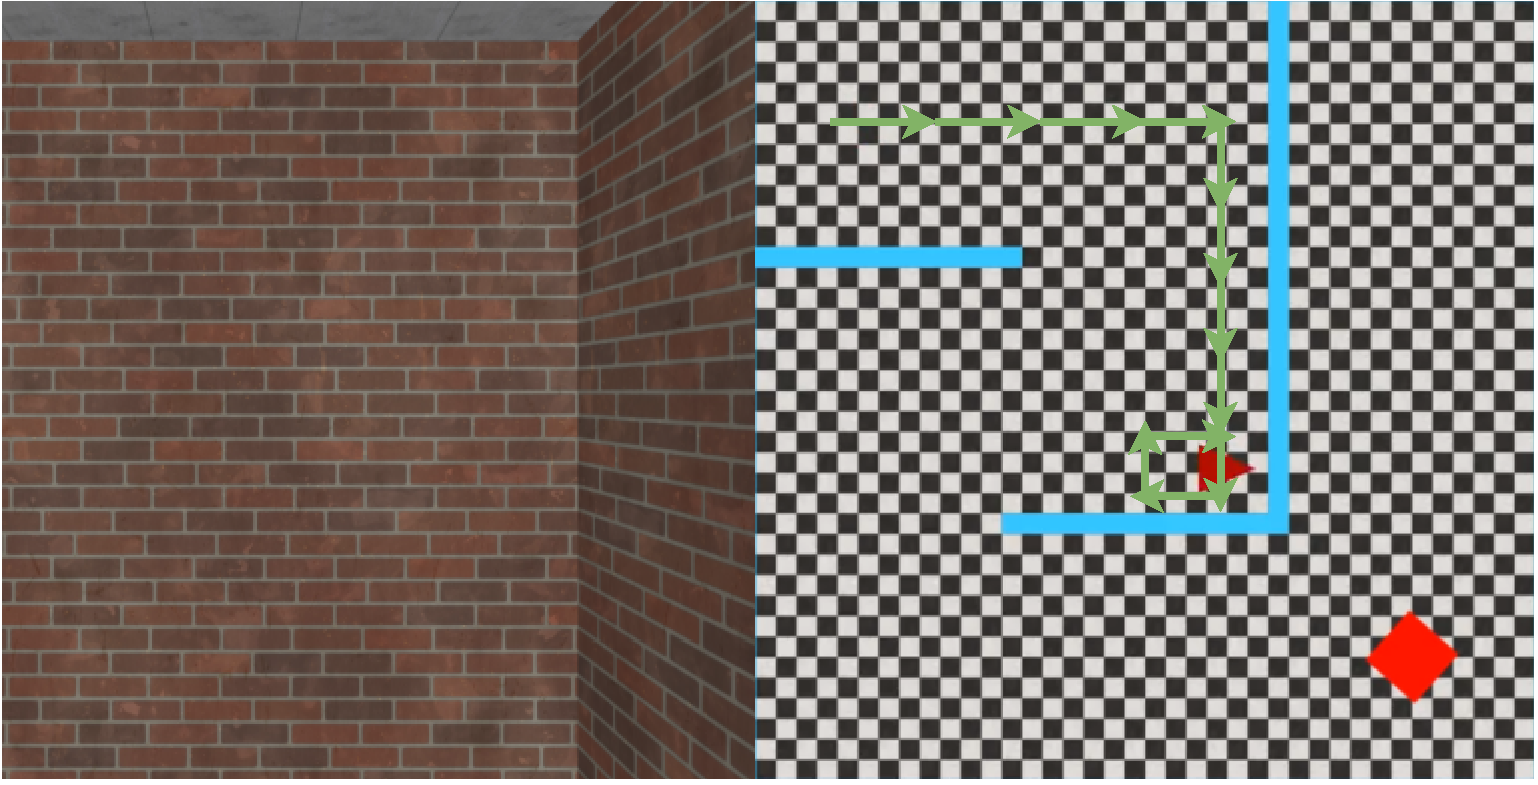
\includegraphics[width=\textwidth]{figures/understanding_vsn/qualitative_results/fail}
        \caption{Failure case.}
        \label{fig:maze_qualitative_fail}
    \end{subfigure}
    \hfill
    \begin{subfigure}[b]{0.49\textwidth}
        \centering
        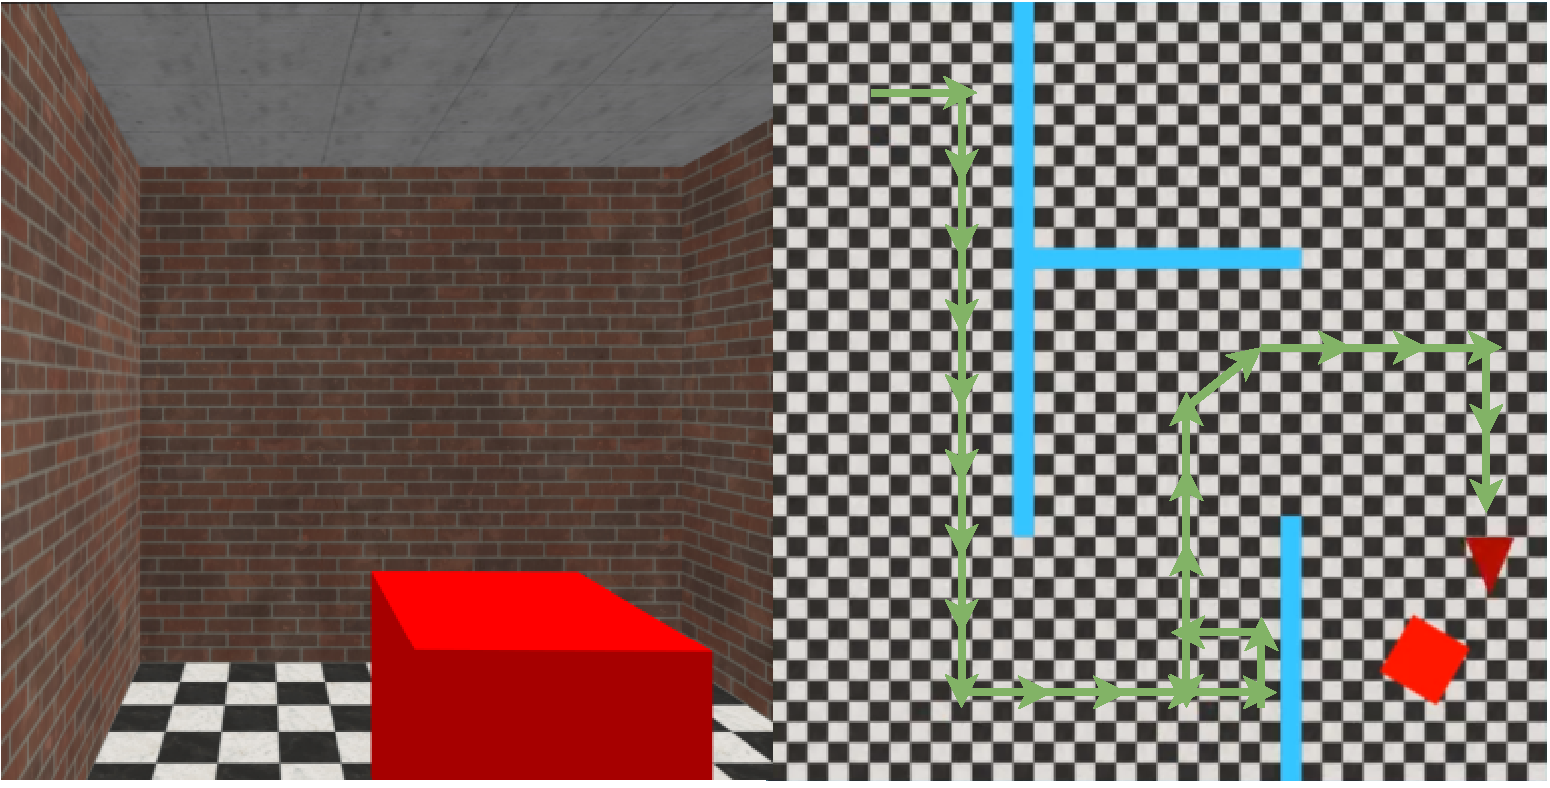
\includegraphics[width=\textwidth]{figures/understanding_vsn/qualitative_results/success}
        \caption{Success case.}
        \label{fig:maze_qualitative_success}
    \end{subfigure}~\caption{\textbf{Qualitative results for Miniworld-Maze agent.} The agent final state and trajectory are shown for a fail case (\ref{fig:maze_qualitative_fail}) and a success case (\ref{fig:maze_qualitative_success}). In the success case, $\epsilon\text{-}greedy$ forces the agent to select a random action, thus exploring the environment, escaping the corner and finally reaching the target.}
    \label{fig:maze_qualitative}
\end{figure}

\subsection{Habitat results}\label{subsec:habitat-results}
Experiments in the Habitat benchmark enable to assess how an agent would act in a more realistic scenario than the one presented by the mazes.
The agent has to navigate through the 3D-scanned scene shown in figure~\ref{fig:dollhouse}.
The agent is initialized from random positions and aims to locate one of the chairs present in the environment.

Figure~\ref{fig:reward-habitat-results} shows the reward obtained by the agent during the training process.
The first million steps correspond to an early stage of exploration.
Then, the reward quickly grows until the agent behavior becomes stable after 3 million steps.

Table~\ref{tab:results-habitat} shows a comparison between the best agent under the same two different output options as in the previous experiment ( $\epsilon\text{-}greedy$ with $\epsilon=0.2$ and \textit{stochastic}), and a random agent as a control case.
Results show how the $\epsilon\text{-greedy}$ approach reports a success rate of $96\%$, while the $\text{stochastic}$ output approach only reaches the target $73\%$ of the times.

Figure~\ref{fig:habitat_qualitative} provides qualitative results for the agent.
It shows the final state (left image) and the top view with the agent's trajectory in blue.
These figures clearly show how in both cases a different valid goal is reached (the agent reaches two different chairs) and how the $\epsilon\text{-greedy}$ strategy leads the agent to do coarser movements.

\begin{table}
    \begin{tabular}{c c c c c c}
        \toprule
        Output type                       & Success                  & \acrshort{spl}                       & \acrshort{dtg}                       & \acrshort{spe}                           & Reward                   \\
        \midrule
        Best agent $+\; \epsilon\text{-}greedy$ & \textbf{0.96 $\pm$ 0.19} & \textbf{$0.66 \pm 0.25$}  & \textbf{$0.25 \pm 0.85$}   & \textbf{189.99 $\pm$ 116.97} & \textbf{4.96 $\pm$ 1.99} \\
        Best agent $+\; stochastic$             & $0.73 \pm 0.45$          & $0.58 \pm 0.36$          & $0.63 \pm 1.17$          & $231.23 \pm 188.13$          & $3.52 \pm 3.90$          \\
%        Ours $+\; deterministic$          & $0.13 \pm 0.33$         & $0.12 \pm 0.30$  $ $2.72 \pm 1.57$   & $432.57 \pm 161.40$          & $-2.03 \pm 3.84$         \\
        $random$                          & $0.05 \pm 0.22$          & $0.02 \pm 0.10$          & $4.49 \pm 1.72$          & $495.50 \pm 26.96$           & $-4.68 \pm 2.16$         \\
        \bottomrule
    \end{tabular}
    \caption{\textbf{Best agent performance on 100 test episodes in Habitat.} The $\epsilon\text{-greedy}$ output mode reports the best results.}
    \label{tab:results-habitat}
\end{table}

\begin{figure}
    \centering
    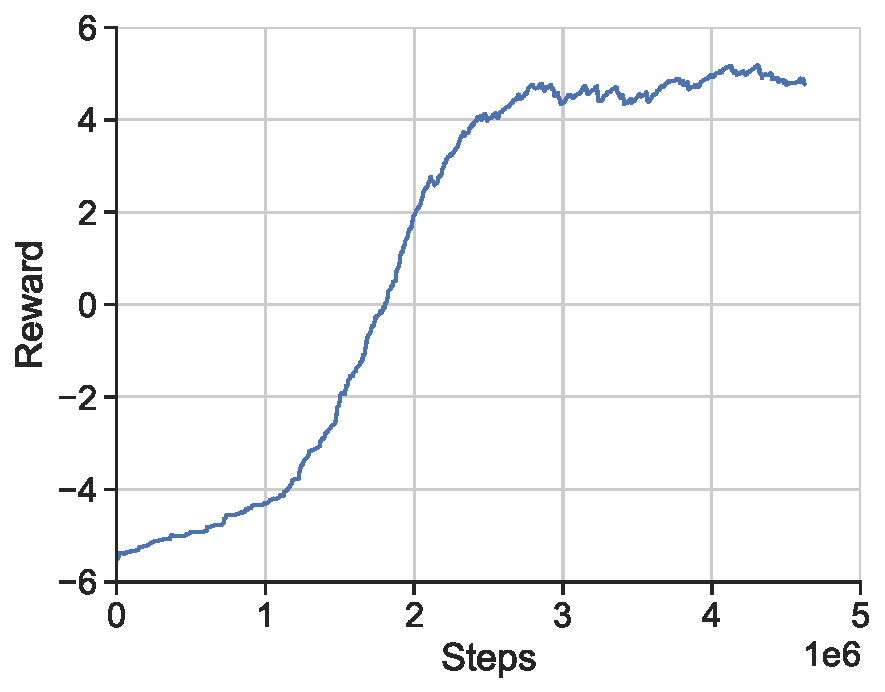
\includegraphics[width=0.8\linewidth]{figures/understanding_vsn/habitat_reward}
    \caption{\textbf{Learning curve of Habitat experiment.} This curve shows how the agent starts with a suboptimal policy, receiving low rewards around $-5$. Then, the rewards increase until a value around 5, once the agent gets an optimal policy.}
    \label{fig:reward-habitat-results}
\end{figure}

\begin{figure}
    \centering
    \begin{subfigure}[b]{0.49\textwidth}
        \centering
        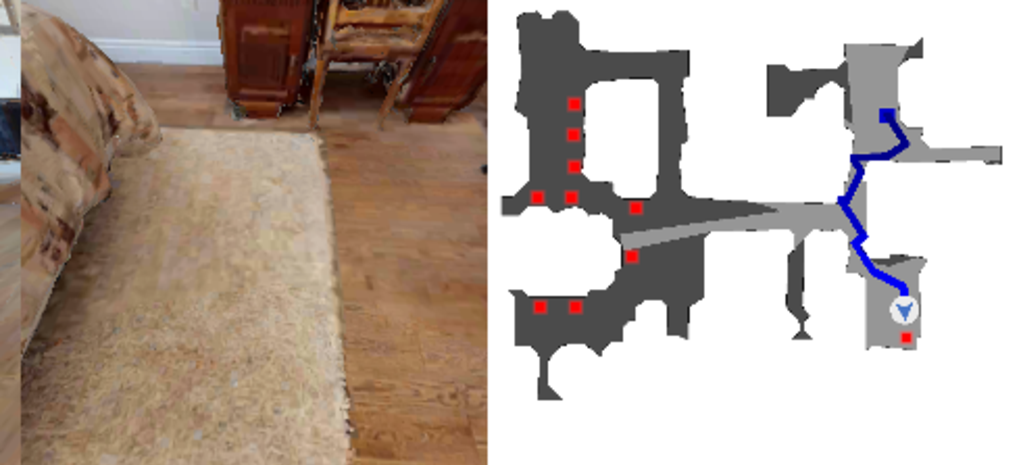
\includegraphics[width=\textwidth]{figures/understanding_vsn/qualitative_results/habitat_epsilon}
        \caption{$\epsilon\text{-greedy}$ output.}
        \label{fig:habitat_qualitative_epsilon}
    \end{subfigure}
    \hfill
    \begin{subfigure}[b]{0.49\textwidth}
        \centering
        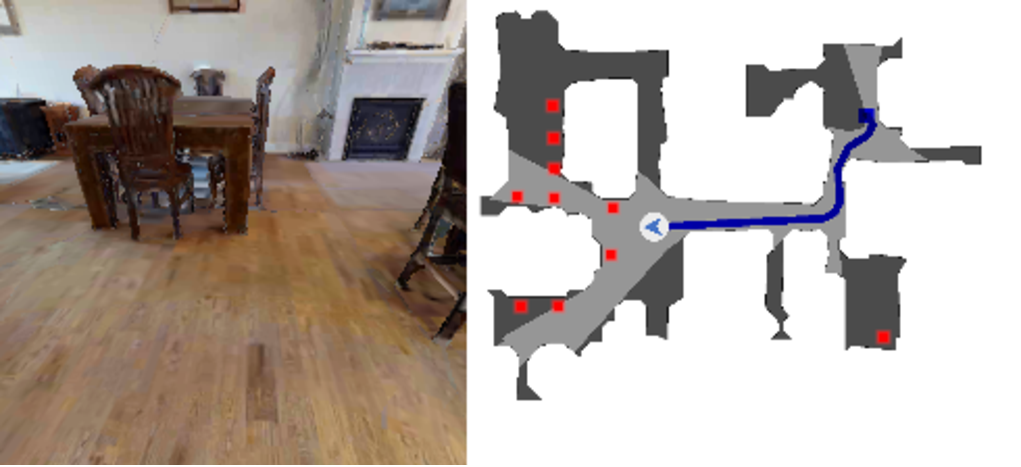
\includegraphics[width=\textwidth]{figures/understanding_vsn/qualitative_results/habitat_stochastic}
        \caption{$Stochastic$ output.}
        \label{fig:habitat_qualitative_stochastic}
    \end{subfigure}~\caption{\textbf{Qualitative results for Habitat agent.} The agent final state and trajectory are shown on the scene using $\epsilon\text{-greedy}$ with $\epsilon = 0.2$ (\ref{fig:habitat_qualitative_epsilon}) and $stochastic$ output (\ref{fig:habitat_qualitative_stochastic}). Note that the $stochastic$ output produces a smother trajectory.}
    \label{fig:habitat_qualitative}
\end{figure}

\begin{figure}
    \centering
    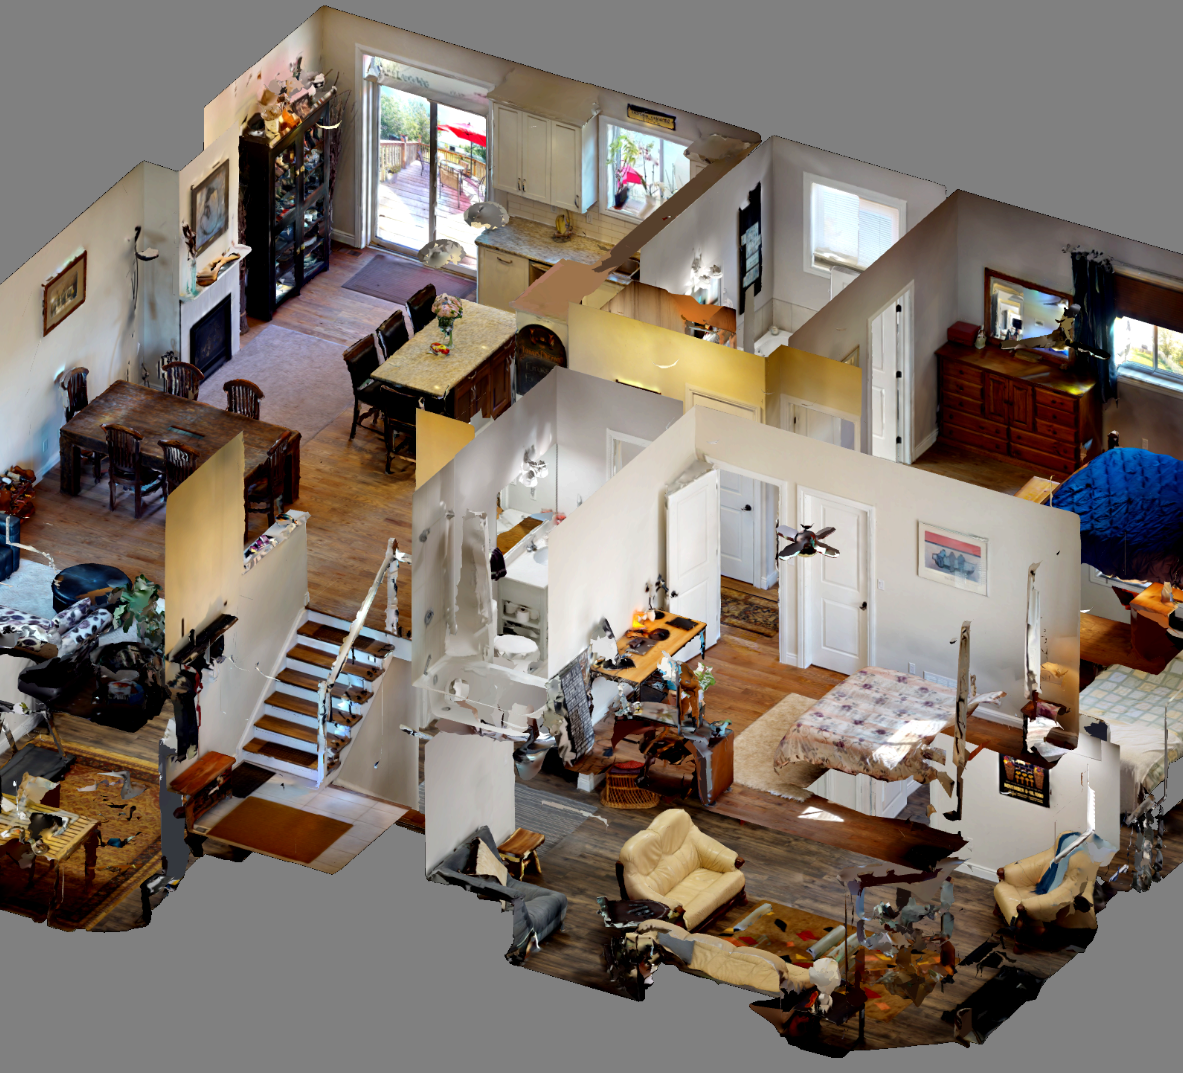
\includegraphics[width=0.6\linewidth]{figures/understanding_vsn/dollhouse}
    \caption{\textbf{Scene 00744-1S7LAXRdDqK from HM3D dataset.} Scene used for Habitat experiments.}
    \label{fig:dollhouse}
\end{figure}


\section{Conclusions}
\label{sec:conclusions}

This chapter presents a thorough experimental evaluation setup for the \acrshort{vsn} problem based on the open-source pyRIL library and two navigation environments: Miniworld-Maze; and a 3D-scanned scene from HM3D database using Habitat simulator.
Following this proposal, a detailed analysis of a state-of-the-art \acrshort{vsn} model based on a \acrshort{clip} feature extractor and \acrshort{lstm}s encoders for the agent state is provided, introducing also reward shaping and $\epsilon\text{-}greedy$ techniques.
The results confirm the impact of these techniques in both environments.

The experimental findings demonstrate that while current \acrshort{vsn} models can achieve promising results in controlled simulation environments, several challenges remain when transitioning to real-world applications.
The success rates achieved in the Miniworld-Maze environment (75\% for S3 and 18\% for S5) and Habitat (96\%) highlight both the potential and limitations of current approaches.
The necessity of exploration strategies such as $\epsilon\text{-}greedy$ and reward shaping techniques underscores the complexity of the navigation problem and the sparse reward challenge inherent in these tasks.

These simulation-based results raise important questions about the practical deployment of \acrshort{vsn} models in real robotic systems.
The gap between simulated and real-world performance, known as the sim-to-real transfer problem, represents a critical challenge that must be addressed for practical applications.
The next chapter explores this challenge by introducing ROS4VSN, a comprehensive framework that enables the deployment and evaluation of \acrshort{vsn} models on real robotic platforms, providing insights into the performance differences between simulation and reality.

The models, data and codes are publicly available at \url{https://github.com/gramuah/vsn} to encourage further research on \acrshort{vsn}\@.